\chapter{Conclusion}
\section{Overall Effect of Spatial Randomness}
\subsection{Logistic Map}
The spatially random processes appear to have stabilized the logistic
map in regions that were otherwise known to be chaotic.
\subsection{Circle Map}

\section{Future Work}
\subsection{Dynamic Load Balancing on the Janus Supercomputer}
We explored and simulated the spatially random logistic map using the
dynamic load balancing tool on Janus\footnote{Janus has 1368 compute nodes, and
  each node has 12 processors. Each processor is capable of
  independently carrying
  out a series of computations.}, the University of Colorado's supercomputer
\cite{janus}. The recursive nature of the map prevents the individual
calculations of an orbit from being parallelized, but a set of
iterations may be load balanced over many
cores. Improvements to this project include: adapting the program to
produce other types of plots, extending the program to model
the Arnold Circle Map, and optimizing the post-simulation data processing. 

A load balancer is a tool that dynamically reassigns tasks as the
processors complete their work. There are many strategies for load
balancing, such as sender initiated diffusion, receiver initiated
diffusion, hierarchical balance model, etc.~\cite{dlb}. The Load
Balance tool on Janus uses a master-slave strategy for
balancing~\cite{janus}. In general, a load balancer recognizes the
number of processors that are going to be used in a simulation, and manages
the workload distribution among them. If, for example, Processor A finishes its load early
(perhaps its initial condition led to near-immediate convergence),
the load balancer assigns Processor A more work by reducing the
load on Processor B, a processor taking more time to complete its
task, and passing it to Processor A.

Figure~\ref{fig:lbtool} demonstrates an example of a simulation
using 40 nodes on Janus. A more detailed explanation of how the load
balancing tool was called on each node is available in
Appendix~\ref{lbdetails}. 
\begin{figure}[H]\linespread{1}   
\caption[Load Balancing Tool Overview]{Load Balancing Tool Overview:
  The load balancer is invoked over 40 nodes, where each node handles
  some value of $r \in [0,4]$ and a number $N_x$ of initial conditions
  $x_0 \in [0,1]$ are tested. Each node produces a datafile, which is
  compiled with the other results to create a bifurcation diagram or
  histogram of periodic orbits.}\label{fig:lbtool}
	\begin{center}
          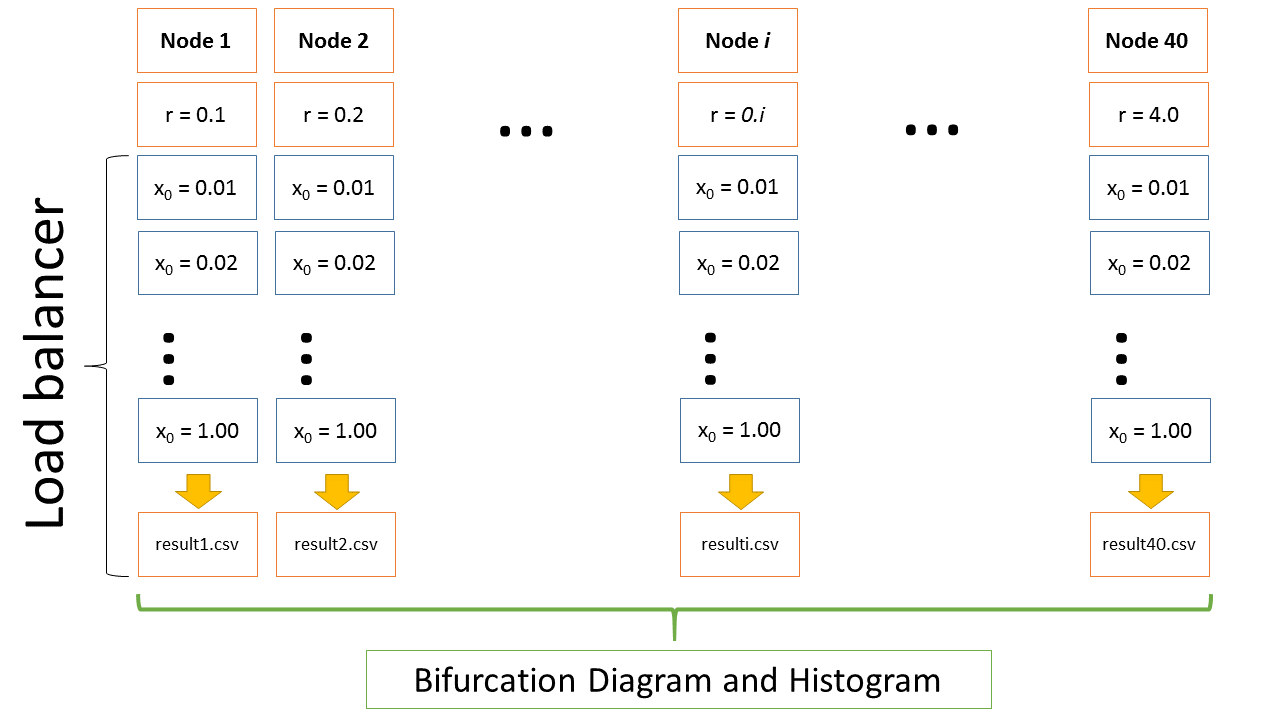
\includegraphics[scale=0.45]{figs/load_balancer.png}
	\end{center}
\end{figure}

The original simulation was written in serial code in
MATLAB, and had extremely variable runtimes (due to the nature of fixed
point iteration). The original version of the code was rewritten for efficiency,
speed, and scalability. The new implementation, written in C++ and
Python, was capable of reproducing two types plots: histograms of observed periodic
orbits and bifurcation diagrams for varying values of the correlation
length, $L$. Figure~\ref{fig:workflow} is a workflow of the
program structure. A more detailed explanation of the scripts in
Figure~\ref{fig:workflow} is in the Appendix~\ref{lbdetails}. 
\begin{figure}[H]\linespread{1}
\caption[Load Balancing Workflow]{Load Balancing Workflow: The load
  balancing tool on Janus takes as input a list of commandline prompts
  (created by \texttt{generate\_cmdline}) calling the
  executable files \texttt{myfunc} and
  \texttt{generate\_rands}. \texttt{generate\_cmdline}
  specifies the parameters the user intends to test for the
  simulation. Each node produces a file called \texttt{result},
  which is parsed by \texttt{Unique} and \texttt{csv2hdf5} to get
  a set of unique orbits to store in a HDF5 file. \texttt{Unique} also creates the histogram. The final script, \texttt{plotbif}, generates the bifurcation diagram.}\label{fig:workflow}
	\begin{center}
          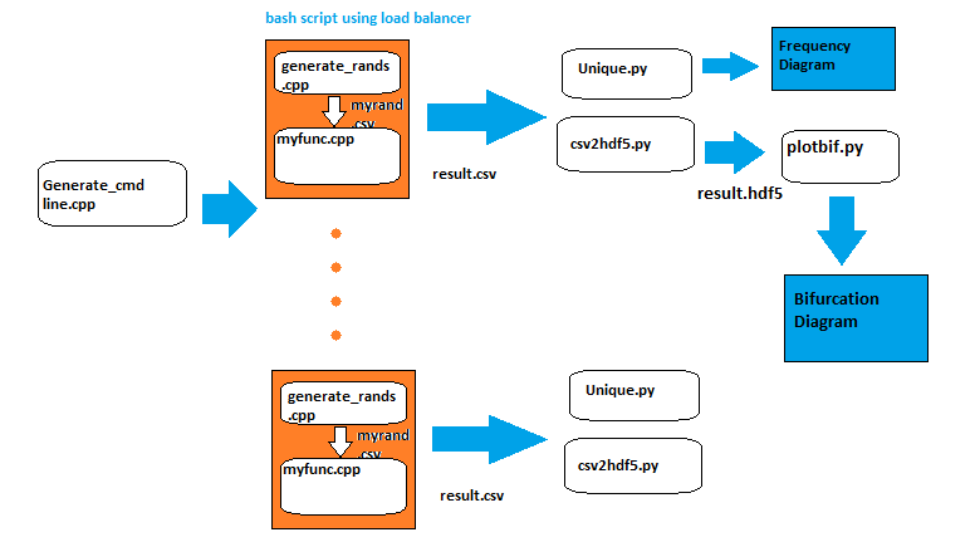
\includegraphics[scale=0.5]{figs/workflow.png}
	\end{center}
\end{figure}

Single core optimization techniques, such as SIMD loop
vectorization and function inlining, as well as using a dynamic load
balancer for more efficient work distribution were
applied. Appendix~\ref{lbdetails} enumerates the modifications applied
to the original implementation. The HDF5
file format was used to store the simulation results in a better
archival format. 

The benchmarking (strong scaling study) results imply
the best speedup and efficiency is gained when invoking the load balancer on
one node (12 processors), although we tested our simulation over 16 nodes
(192 processors). 
\begin{figure}[!h]
\caption[Impact of the load balancing tool: Efficiency and
Speedup]{Efficiency (left) and Speedup (right) of the new
  implementation. The best efficiency occurred for one node, and the best speedup was also achieved for 1 node.}\label{fig:effsp}
\centering
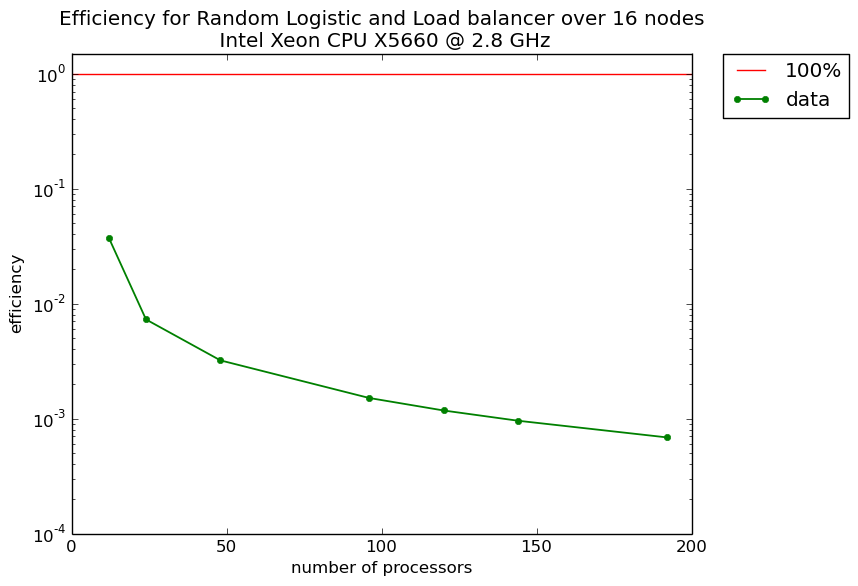
\includegraphics[width=.5\textwidth]{figs/efficiency_random_logistic.png}\hfill
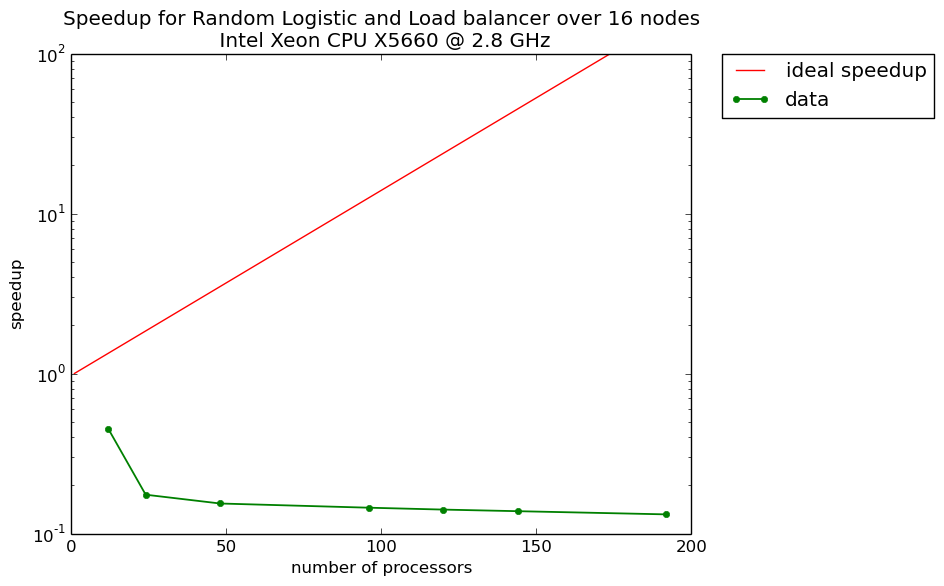
\includegraphics[width=.5\textwidth]{figs/speedup_random_logistic.png}
\end{figure}